\chapter{Non-Relativistic Solution of the Hydrogen Molecular Ion in 2 Spatial Dimensions}

\section{Existing Solutions}

We apply similar method used in the 3D case of the $ H_2^{+} $ ion to find the solution in 2 dimensions. The problem itself is analogous to the 3D problem, but leads to the Mathieu's function as the solution for the radial problem.

There are not too many papers dealing with solving the $ H_2^{+} $ but here is some relevant, and recent work in this problem. In addition to the Bates paper \cite{Bates1}, there are other, more recent papers \cite{H2Plus2d1} \cite{TwoCentersParticle}, \cite{Kolos} which deal with the solution of the Schrodinger equation and spectrum of the $ H_2^{+} $ molecule in 3 dimensions.  As with other work in this problem, the paper relies on the work done by Bates et all. \cite{Bates1}. The solution in \cite{H2Plus2d1} agrees well with our solution.  One can also apply approximate methods, but they should be considered inferior to the analytical solution, we provide here. 

Analogous to the 3D case, we rely on Born-Oppenheimer (BO) approximation, in order to provide an analytical solution. The same justification for using the BO approximation in 3D molecular systems applies to the 2D problems as well, since the masses of the nuclei and electron(s) remain unchanged.  Following the same BO approximation as in Chapter 1, and using atomic units, the Schrodinger equation for the $ H_2^{+} $ molecules is given by equation \eqref{eqPartial2D} below. 


\begin{equation}\label{eqPartial2D}
\left(-\frac{1}{2}\nabla^2-\frac{1}{r_a}-\frac{1}{r_b}\right)\psi = E\,\psi
\end{equation}

The equation \eqref{eqPartial2D} is superficially similar to the equation \eqref{eqPartial3D} and the diagram \ref{h2ion3d}, but in this case, the $ r_a $ and $ r_b $ represent the nuclei coordinates in 2 dimensions.

Following the \cite{2DHAtom}, The electron wavefunction depends on only 3 quantum numbers, principal quantum number $ n $, angular quantum number $ l $ and spin $ s $. Again we ignore the spin degrees of freedom, considering the electron to be the regular 3 dimensional particles, where only its orbit is restricted to 2 dimensions.  Therefore the spin magnetic moment of the electron is not affected by the 2D restriction and the spin vector can point in any direction in 3D space. Also the orbit can have different shapes, thus there remains the need for an orbital quantum number. However, there can be one one orientation of the orbit, thus we do not consider the magnetic quantum number. This reasoning agrees with the solution of the electron wavefunction to the hydrogen atom in 2 dimensions \cite{H2atom} where electron wavefunction solution only depends on the principal and orbital quantum numbers.

The geometry of the 2D problem leads to choosing the elliptical coordinates (as in 3D problem), with two coordinates, $ \mu $ and $ \lambda $ denoting the position of the electron in 2D plane. \cite{Arfken}

\section{Exact solution of the electron energies of the \texorpdfstring{$ H_2^+ $}{$H_2^+$} molecule}

The goal is to provide the exact solution to the wavefunction of the $ H_2^{+} $ electron, for a given definition of exact. However even for this, relatively simple problem, it is impossible to find a closed form solution. So the solution is exact, in the sense that it can be done to an arbitrary precision.

As illustrated by the figure  \ref{h2ion2d}, we express equation \eqref{eqPartial2D} in the elliptical coordinates, and by setting the $ x $ axis to be perpendicular to the inter-nuclear axis, we have the nuclei at: $ z = \pm \frac{R}{2}  $, R being the distance between nuclei. So in  2D elliptic coordinates, $ \lambda $, $ \mu $ we have:

\begin{equation}\label{variables1}
r_a = \frac{R}{2}\left(\lambda + \mu \right)\,\,\,\,\,\,\,\,\,\,\,\,\,\,\,\,\,\,\,\,\,\, r_b = \frac{R}{2}\left(\lambda - \mu \right)
\end{equation}
so
\begin{equation}\label{variables1a}
\lambda = \left(r_a + r_b\right)/R;\,\,\,\,\,\,\,\,\,\,\,\,\,\,\,\,\,\,\mu =  \left(r_a - r_b\right)/R
\end{equation}
\begin{equation}
\text{where } \lambda \in \left[1,\infty\right]\,,\,\,\,\,\,\,\,\,\,\mu \in \left[ -1, 1 \right]
\end{equation}

Now if we plug in the \eqref{variables1} into \eqref{eqPartial2D} we get by using $ \nabla $ in 2D elliptic cylindrical coordinates \cite{MorseFeshbach} .
\begin{equation}
\begin{split}
& \nabla^2 = \frac{4}{ R^2 (\lambda^2-\mu^2) }\left[ \sqrt{\lambda^2-1}\frac{\partial}{\partial \lambda}\left(\sqrt{\lambda^2-1}\frac{\partial \psi}{\partial \lambda} \right) +
\sqrt{1-\mu^2}\frac{\partial}{\partial \mu}\left(\sqrt{1 - \mu^2}\frac{\partial \psi }{\partial \mu }\right) \right] = \\
& \frac{4}{ R^2 (\lambda^2-\mu^2) }\left[(\lambda^2-1)\frac{\partial^2 \psi}{\partial \lambda^2} + \lambda\frac{\partial \psi}{\partial \lambda} + (
1 - \mu^2)\frac{\partial^2 \psi}{\partial \mu^2} - \mu\frac{\partial \psi}{\partial \mu} \right]
\end{split}
\end{equation}

So the equation transforms to (with $ \psi = \psi(\lambda, \mu) $:
\begin{equation}\label{SchrFull-1}
-\frac{1}{2}\frac{4}{ R^2 (\lambda^2-\mu^2) }\left[(\lambda^2-1)\frac{\partial^2 \psi}{\partial \lambda^2} + \lambda\frac{\partial \psi}{\partial \lambda} +
(1 - \mu^2)\frac{\partial^2 \psi}{\partial \mu^2} - \mu\frac{\partial \psi}{\partial \mu} \right] - \frac{4}{R}\frac{\lambda}{\lambda^2-\mu^2}\psi = E \psi
\end{equation}

We assume that the total electronic wavefunction can be written as the product of two functions:
\begin{equation}\label{variables2}
\begin{split}
& \psi(\lambda,\mu) = F(\mu)L(\lambda)
\end{split}
\end{equation}

\begin{figure}
 \captionsetup{type=figure}
  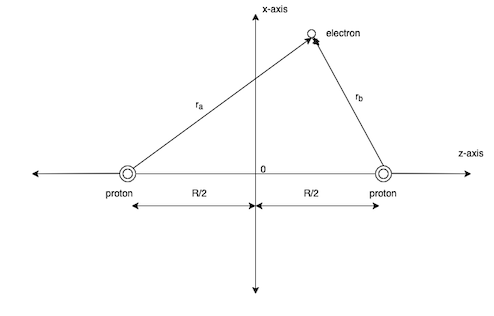
\includegraphics{H2Ion3D-2.png}
  \caption{Hydrogen Ion in 2 dimension} 
  \label{h2ion2d}
\end{figure}
it follows:
\begin{equation}
\begin{split}
& \frac{2}{ R^2 (\lambda^2-\mu^2) }\left[(\lambda^2-1)F\frac{\partial^2 L}{\partial \lambda^2} + \lambda F\frac{\partial L}{\partial \lambda} +
(1 - \mu^2)L\frac{\partial^2 F}{\partial \mu^2} - \mu L\frac{\partial F}{\partial \mu} \right] + \frac{4}{R}\frac{\lambda}{\lambda^2-\mu^2} F L + E F L = 0 \Rightarrow \\[.8em]
& (\lambda^2-1)\frac{1}{L}\frac{\partial^2 L}{\partial \lambda^2} + \frac{\lambda}{L}\frac{\partial L}{\partial \lambda} +
(1 - \mu^2)\frac{1}{F}\frac{\partial^2 F}{\partial \mu^2} - \frac{\mu}{F} \frac{\partial M}{\partial \mu} + 2R\lambda + \frac{R^2}{2} E (\lambda^2 - \mu^2) = 0
\end{split}
\end{equation}

We can conclude that both equations for $ \lambda $ and $ \mu $ must be equal to the separation constant $ A $. 
\begin{equation}\label{eqLG3}
\begin{split}
& (\lambda^2-1)\frac{\partial^2 L}{\partial \lambda^2} + \lambda\frac{\partial L}{\partial \lambda} + \left(2R\lambda -  \frac{R^2}{2} E\lambda^2\right) L = AL \\[.8em]
& (1 - \mu^2)\frac{\partial^2 F}{\partial \mu^2} - \mu\frac{\partial F}{\partial \mu} - \frac{R^2}{2} E \mu^2 F = -AF
\end{split}
\end{equation}
where $ A $ is the separation constant.

\subsection{Algebraic Solution}

\subsubsection{ M Equation }

Using the substitution $ \mu  = \cos x$ and $ F(\mu) = M(x) $ we get a new equation:

\begin{equation}\label{M2}
\frac{d^2 M}{d x^2} + \left[-A + \frac{p^2}{2} + \frac{p^2}{2}\cos(2x) \right]M = 0 
\end{equation}

The equation \eqref{M2} can be written as:

\begin{equation}\label{M2a}
\frac{d^2 M}{d x^2} + \left[w - 2q\cos(2x)\right]M = 0
\end{equation}
where
\begin{equation}
\begin{split}
& w = - A + \frac{p^2}{2} \\[.7em]
& q = - \frac{p^2}{2}
\end{split}
\end{equation}

The equation \eqref{M2a} is a form of a  Mathieu's equation \cite{Mathieu2}. 

From the geometry of the problem we conclude that $ M(\mu) $ must be an even function.  Following \cite{Mathieu4} we look for the solution as class I and class II, which has even and odd eigenvalue functions as:
\begin{equation}
\begin{split}
V_0 = \cfrac{2}{V_2 - \cfrac{1}{V_4 - \cfrac{1}{V_6 - ...}}}\label{V-1-1}
\end{split}
\end{equation}
\begin{equation}
\begin{split}
V_1 - 1 = \cfrac{1}{V_3 - \cfrac{1}{V_5 - \cfrac{1}{V_7 - ...}}}\label{V-1-2}
\end{split}
\end{equation}
where 
\begin{equation}
V_m = \frac{w - m^2}{q}
\end{equation}

The equations \ref{V-1-1} and \ref{V-1-2} provide the first gen equation for the even and odd solution respectively.

\subsubsection{ F Equation }

\begin{equation}\label{eqLG3}
(\lambda^2-1)\frac{\partial^2 F}{\partial \lambda^2} + \lambda\frac{\partial F}{\partial \lambda} + \left(2R\lambda -  \frac{R^2}{2} E\lambda^2\right) F = -AF
\end{equation}

We observe that both equations for the functions $ M(\mu) $ and $ F(\lambda) $ are either exact match or related to the Mathieu's equations. In general the Mathieu's equation represents the standing wave on an elliptical drum, (2D space), and the solution for the time independent Schrodinger equation is in general a standing wave, in 2D in this case. So it is plausible that these types of solutions are similar.

There are actually two ways to try to solve this equation. One would be a brute force, by using some orthogonal polynomial (Laguerre) and looking for the eigenvalues.

The Laguerre approach seems to be numerically unstable. The algorithm is fast but the results are only good to the order of magnitude. 

The second is a bit more algebraic, and likely more accurate.

Following \cite{Bates1} and \cite{H2Plus2d2} we could look for the solution in the form of:
\begin{equation}\label{eqLsumG}
L(\lambda) = \left(\lambda +1\right)^\sigma e^{-p\lambda}\sum_{n=0}^{\infty}{a_nx^n}
\end{equation}
where we use the substitution
\begin{equation}\label{eqLG}
\begin{split}
\sigma = \frac{R}{p} - \frac{1}{2}
\end{split}
\quad\text{ and }\quad
\begin{split}
x = \frac{\lambda-1}{\lambda+1}
\end{split}
\end{equation}
Substituting \eqref{eqLG} into \eqref{eqLsumG} and after some formidable algebra, we get a recurrence relation:
\begin{equation}
\alpha_na_{n+1}-\beta_n a_n+\gamma_na_{n-1} = 0\,\,\,\,\,n \ge 0
\end{equation}
with
\begin{equation}
\begin{split}
& \alpha_n = \left(n + 1\right)\left(n + \frac{1}{2}\right)\\[.8em]
& \beta_n = \left[2n^2 + (4p - 2\sigma)n - A + p^2 - 2p\sigma - \frac{\sigma}{2}\right] \\[.8em]
& \gamma_n = (n-1)\left(n - 2\sigma - \frac{1}{2}\right) + \sigma\left(\sigma - \frac{1}{2}\right)
\end{split}
\end{equation}
and if follows that
\begin{equation}
\begin{split}
\frac{a_n}{a_{n-1}} = F_n
\end{split}
\quad\text{ where }\quad
\begin{split}
F_n = \cfrac{\gamma_n}{\beta_n - \cfrac{\alpha_n \gamma_{n+1}}{\beta_{n+1}-\cfrac{\alpha_{n+1}\gamma_{n+1}}{\beta_{n+1}-\text{...}}}}
\end{split}
\end{equation}
Since $ a_{-1} = 0$ we have
\begin{equation}
\frac{\beta_0}{\alpha_0} = F_1
\end{equation}

The Mathematica code is in appendix C. The energies calculated and the plot of the potential for the states $1s_g^{+}$ and $ 2p_u^{+} $ are in the tables below.

The states  $ 1s_g $ and $ 2p_u^{+} $ represent the Gerade ground state and the Ungerade state respectively.

    \begin{table}[h!]
  \caption{ The separation constant A, electronic energy E}{total energy $ E + \frac{1}{R} $ , for the state $ 1s_g $ some values of the inter-nuclear separation R }
  \centering
  \label{1sg}
		\begin{tabular}{ m{6em} m{6em}  m{6em}  m{6em} m{6em} }
			\hline
			R & E & $ E + \frac{1}{R} $ & A & p \\ \hline \hline
 0.2 & -6.50361 & -1.50361 & 19.2757 & 0.360655\\
 0.3 & -5.81983 & -2.48649 & 175.774 & 0.511754\\
 0.4 & -5.27552 & -2.77552 & 198.466 & 0.649647\\
 0.5 & -4.83822 & -2.83822 & 218.834 & 0.777674\\
 0.6 & -4.48148 & -2.81482 & 30.6031 & 0.898146\\
 0.7 & -4.18616 & -2.75759 & 255.124 & 1.01272\\
 0.8 & -3.93852 & -2.68852 & 271.721 & 1.12264\\
 0.9 & -3.72861 & -2.6175 & 287.554 & 1.22886\\
 1. & -3.54905 & -2.54905 & 302.754 & 1.33211\\
 1.1 & -3.39429 & -2.4852 & 317.417 & 1.43302\\
 1.5 & -2.95083 & -2.28416 & 371.99 & 1.822\\
 2. & -2.63638 & -2.13638 & 433.864 & 2.29625\\
 2.5 & -2.4621 & -2.0621 & 491.12 & 2.77382\\
 3. & -2.36086 & -2.02752 & 545.139 & 3.25943\\
 3.5 & -2.29797 & -2.01225 & 596.728 & 3.75167\\
 4. & -2.25565 & -2.00565 & 646.407 & 4.24796\\
 4.5 & -2.22496 & -2.00274 & 694.536 & 4.74634\\
 5. & -2.20134 & -2.00134 & 741.373 & 5.24564\\
 6 & -2.16637 & -1.9997 & 16608. & 6.24457\\
 7 & -2.14043 & -1.99757 & 919.107 & 7.24158\\
 8 & -2.11874 & -1.99374 & 1003.68 & 8.23405\\
 9 & -2.09856 & -1.98745 & 1086.12 & 9.21909\\
 10 & -2.07822 & -1.97822 & 1166.79 & 10.1937 \\
          \hline
		\end{tabular}
    \end{table}

\begin{table}[h!]
  \caption{ The separation constant A, electronic energy E}{ total energy $ E + \frac{1}{R} $ , for the state $ 2p_u^{+} $ for some values of the inter-nuclear separation R } 
  \centering
  \label{2sg}
		\begin{tabular}{ m{6em} m{6em}  m{6em}  m{6em} m{6em} }
			\hline
			R & E & $ E + \frac{1}{R} $ & A & p  \\ \hline \hline
  0.2 & -0.841481 & 4.15852 & 33.4451 & 0.129729\\
  0.3 & -0.911818 & 2.42152 & 39.6245 & 0.202563\\
  0.4 & -1.03317 & 1.46683 & 44.6816 & 0.287495\\
  0.5 & -1.20111 & 0.798885 & 49.0907 & 0.387478\\
  0.6 & -1.39266 & 0.274004 & 53.0632 & 0.500679\\
  0.7 & -1.58212 & -0.153551 & 56.7159 & 0.622591\\
  0.8 & -1.75267 & -0.502667 & 395.73 & 0.748901\\
  0.9 & -1.89725 & -0.786142 & 417.783 & 0.876577\\
  1. & -2.01521 & -1.01521 & 66.3746 & 1.0038\\
  1.1 & -2.10899 & -1.1999 & 459.254 & 1.12957\\
  1.5 & -2.31161 & -1.64494 & 534.677 & 1.61262\\
  2. & -2.36744 & -1.86744 & 619.719 & 2.17598\\
  2.5 & -2.35029 & -1.95029 & 698.046 & 2.7101\\
  3. & -2.31526 & -1.98193 & 111.724 & 3.2278\\
  3.5 & -2.2797 & -1.99399 & 841.77 & 3.73673\\
  4. & -2.24845 & -1.99845 & 909.103 & 4.24118\\
  4.5 & -2.22222 & -2. & 974.188 & 4.74341\\
  5. & -2.20044 & -2.00044 & 1037.4 & 5.24457\\
  6 & -2.16704 & -2.00038 & 1159.29 & 6.24554\\
  7 & -2.14278 & -1.99992 & 1276.36 & 7.24556\\
  8 & -2.12404 & -1.99904 & 1389.63 & 8.24435\\
  9 & -2.10851 & -1.9974 & 1499.83 & 9.24093\\
  10 & -2.09461 & -1.99461 & 1607.45 & 10.2338\\
		\hline
		\end{tabular}
\end{table}

\begin{figure}
  \includegraphics{H2_1sG-Potential.png}
  \caption{$ H_2^{+} $ Energy and Potential curves for the $ 1s_g^{+} $ state}
\end{figure}

\begin{figure}
  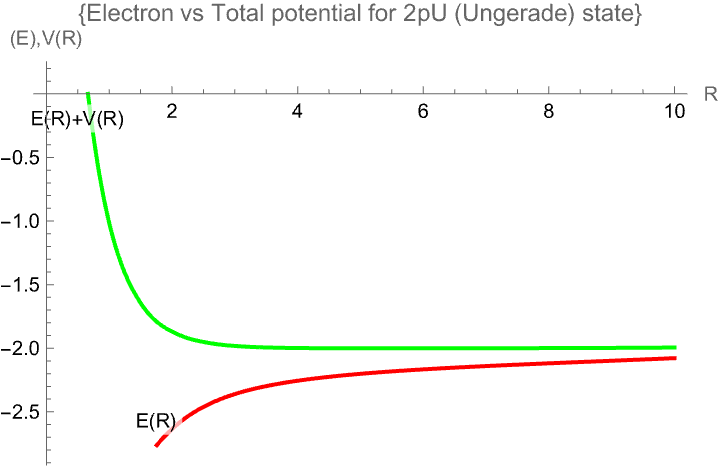
\includegraphics{H2_2pU-Potential.png}
  \caption{$ H_2^{+} $ Energy and Potential curves for the $ 2p_u^{+} $ state}
\end{figure}


\begin{figure}
  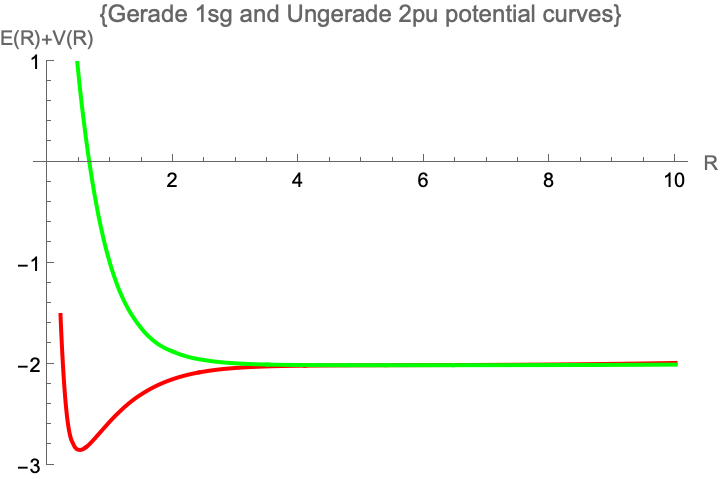
\includegraphics{	H2_sGpU-Potential.png}
  \caption{$ H_2^{+} $ Potential curves for the $ 1s_g^{+}\,\, \text{and}\,\, 2p_u^{+} $ states}
\end{figure}
